\documentclass[tikz,border=6pt]{standalone}
\usepackage{amsmath}
\usetikzlibrary{arrows.meta,calc,patterns,positioning}
\begin{document}

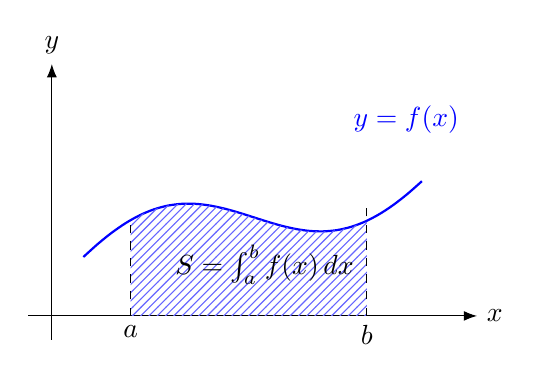
\begin{tikzpicture}[>=Latex,scale=1]
  \draw[->] (-0.3,0) -- (5.4,0) node[right] {$x$};
  \draw[->] (0,-0.3) -- (0,3.2) node[above] {$y$};
  \draw[domain=0.4:4.7,smooth,variable=\x,blue,thick] plot ({\x},{0.35+0.35*\x+0.55*sin(70*\x)});
  \path[pattern=north east lines,pattern color=blue!60]
    (1,0) -- plot[domain=1:4,smooth,variable=\x] ({\x},{0.35+0.35*\x+0.55*sin(70*\x)}) -- (4,0) -- cycle;
  \draw[dashed] (1,0) node[below] {$a$} -- (1,1.15);
  \draw[dashed] (4,0) node[below] {$b$} -- (4,1.45);
  \node at (2.7,0.65) {$S=\int_a^b f(x)\,dx$};
  \node[blue] at (4.5,2.5) {$y=f(x)$};
\end{tikzpicture}

\end{document}
